% TODO: what to put here?
%In this section we summarize the results of the experiments described in Section~\ref{s:exp}.
% In this section we summarize the results of the experiments examining
% the influence of risk group dynamics on simulated epidemics.
% The aim of the experiments was to explore the impact of
% different implementations of risk group dynamics on model outputs
% in a generalized epidemic model.
% We compare the projected incidence and prevalence across
% four model variants and range of turnover magnitudes,
% as well as the estimated TPAF of the high risk group, with and without turnover.
% ==================================================================================================
\subsection{Experiment 1: Influence of turnover on equilibrium incidence and prevalence}
\label{ss:res-1}
First, we present general trends in equilibrium prevalence and incidence
with respect to turnover.
% --------------------------------------------------------------------------------------------------
\paragraph{Experiment 1.1: Overall prevalence with vs without turnover}\label{p:res-turnover-simple}
Figure~\ref{fig:compare-turnover-prevalence} shows
the influence of turnover on overall prevalence at two different treatment rates.
In both scenarios, turnover appeared to slow
the initial epidemic growth as indicated by overall prevalence.
However, at equilibrium, the influence of turnover on overall prevalence
depended on the treatment rate:
prevalence was higher with turnover for $\tau = 0.1$
(Figure~\ref{fig:compare-turnover-prevalence-all-tau=0.1}),
while it was higher without turnover for $\tau = 0.2$
(Figure~\ref{fig:compare-turnover-prevalence-all-tau=0.2}).
Experiments 1.2 and 1.3 aimed to clarify and explain this influence
through exploration of group-specific incidence and prevalence at equilibrium
under different rates of turnover $\phi$ and treatment $\tau$.
\begin{figure}[!tbp]
  \centering
  \begin{subfigure}{0.45\linewidth}
    \centering
    \includegraphics[width=\linewidth]{{sit-turnover-prevalence-all-tau=0.1}.pdf}
    \caption{Treatment rate $\tau= 0.1$}
    \label{fig:compare-turnover-prevalence-all-tau=0.1}
  \end{subfigure}
  \begin{subfigure}{0.45\linewidth}
    \centering
    \includegraphics[width=\linewidth]{{sit-turnover-prevalence-all-tau=0.2}.pdf}
    \caption{Treatment rate $\tau = 0.2$}
    \label{fig:compare-turnover-prevalence-all-tau=0.2}
  \end{subfigure}
  \caption{Overall projected prevalence with and without risk group turnover
    under two different treatment rates $\tau$.}
  \label{fig:compare-turnover-prevalence}
\end{figure}
% --------------------------------------------------------------------------------------------------
\paragraph{Experiment 1.2: Influence of turnover rates on incidence and prevalence}
\label{p:res-turnover-1D}
Figure~\ref{fig:1d-prevalence} illustrates trends in equilibrium prevalence versus turnover
among the high and low risk groups for fixed treatment rate ($\tau = 0.1$).
For both groups, the same profile was observed:
at low turnover, increasing turnover increased prevalence, up to a maximum value (region~A),
and increasing turnover beyond this point (region~B) then decreased prevalence.
In the high risk group (Figure~\ref{fig:1d-prevalence-high}),
this transition occurred at a lower rate of turnover,
while in the low risk group (Figure~\ref{fig:1d-prevalence-low}),
the transition occurred at a higher rate of turnover.
This peaked prevalence profile can be explained by the interaction between two factors:
the movement of individuals between risk groups and incidence.
\begin{figure}[!tbp]
  \centering
  \begin{subfigure}{0.45\linewidth}
    \centering
    \includegraphics[width=\linewidth]{{1d-prevalence-high-tau=0.1}.pdf}
    \caption{High risk}
    \label{fig:1d-prevalence-high}
  \end{subfigure}
  \begin{subfigure}{0.45\linewidth}
    \centering
    \includegraphics[width=\linewidth]{{1d-prevalence-low-tau=0.1}.pdf}
    \caption{Low risk}
    \label{fig:1d-prevalence-low}
  \end{subfigure}
  \caption{Equilibrium prevalence among high and low  risk groups versus turnover,
    as controlled by the duration in the high risk group $\delta_H$.
    Turnover shown in log scale.}
  \label{fig:1d-prevalence}
\end{figure}
\par
The movement of individuals between risk groups is depicted in Figure~\ref{fig:flows}
for four rates of turnover and a simplified system (two risk groups).
Recall that, by our assumptions,
the distribution of health states among individuals leaving a risk group
was equal to the distribution of health states within the group.
Therefore, a higher proportion of individuals leaving the high risk group
were infectious as compared to individuals entering the high risk group,
who were mostly susceptible.
Thus, in the high risk group,
turnover yielded a net replacement of infectious individuals with susceptible individuals.
However, turnover similarly replaced treated individuals
with susceptible individuals in this group.
If incidence is sufficiently high,
infection of these susceptible individuals can
outpace the loss of infectious individuals via turnover.
As a result, prevalence among the high risk group
can actually increase with increasing turnover.
In fact, this is what we observed in this model for moderate rates of turnover
(Figure~\ref{fig:dX-high-I}),
yielding the increase in prevalence among high risk individuals
shown in region~A of Figure~\ref{fig:1d-prevalence-high}.%
%and illustrated in Figure~\ref{fig:flows-med}~vs~\ref{fig:flows-low}.%
\footnote{If prevalence is defined as to include
  both infectious individuals and individuals on treatment,
  such as in the context of HIV,
  then infection prevalence among the high risk group
  monotonically decreased with increasing turnover \citep{Knight2019}.}
Among the low risk group, turnover yielded a net exchange susceptible individuals
for infectious and treated individuals.
As a result, moderate rates of turnover also
increased prevalence among the low risk group,
as shown in region~A of Figure~\ref{fig:1d-prevalence-low}.
%Overall, turnover increases infection prevalence by
%increasing the number of susceptible individuals exposed to the high risk state.
\par
\begin{figure}[!tbp]
  \centering
  \begin{subfigure}[t]{0.6\linewidth}
    \centering
    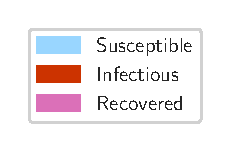
\includegraphics[width=\linewidth]{flows-legend.pdf}
  \end{subfigure}
  \begin{subfigure}[t]{0.2\linewidth}
    \centering
    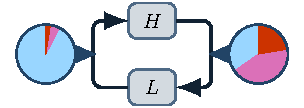
\includegraphics[width=\linewidth]{flows-low.pdf}
    \caption{Low turnover}
    \label{fig:flows-low}
  \end{subfigure}%
  \begin{subfigure}[t]{0.2\linewidth}
    \centering
    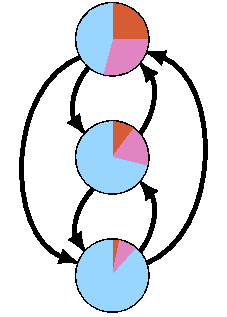
\includegraphics[width=\linewidth]{flows-med.pdf}
    \caption{Moderate turnover}
    \label{fig:flows-med}
  \end{subfigure}%
  \begin{subfigure}[t]{0.2\linewidth}
    \centering
    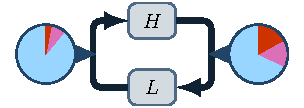
\includegraphics[width=\linewidth]{flows-high.pdf}
    \caption{High turnover}
    \label{fig:flows-high}
  \end{subfigure}%
  \begin{subfigure}[t]{0.2\linewidth}
    \centering
    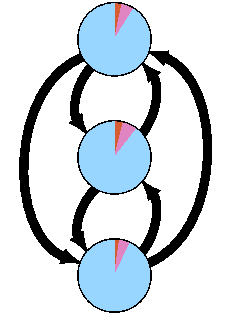
\includegraphics[width=\linewidth]{flows-extreme.pdf}
    \caption{Very high turnover}
    \label{fig:flows-extreme}
  \end{subfigure}
  \caption{Average health states of individuals
    moving between high and low risk groups due to different rates of turnover.}
  \label{fig:flows}
\end{figure}
Next, and in order to explain the reversal of these trends
at higher rates of turnover (region~B),
we examined the second factor in
the influence of turnover on infection prevalence: incidence.
Consider the force of infection equation, Eq~(\ref{eq:foi}).
As shown in Appendix~\ref{aa:eqs-incidence}, the dynamic component in this expression is
the proportion of available partnerships which are offered by infectious individuals,
denoted as $\bm{C}_{\mathcal{I}}$.
This component can be further broken down into the following two sub-factors:
$\hat{C}_{\mathcal{I}}$ the average contact rate among infectious individuals, and
$\hat{\mathcal{I}}$ overall prevalence.
Thus the influence of turnover on incidence
can be understood through the influence of turnover on these two sub-factors.%
\footnote{Since we assumed proportionate mixing among risk groups,
  and only consider heterogeneity in contact rate $C_i$,
  incidence in each risk group is the same as overall
  except for a scale factor proportional to $C_i$.}
\begin{figure}[!tbp]
  \centering
  \begin{subfigure}{0.45\linewidth}
    \centering
    \includegraphics[width=\linewidth]{{1d-C-I-tau=0.1}.pdf}
    \caption{Average contact rate among infectious individuals $\hat{C}_{\mathcal{I}}$}
    \label{fig:1d-C-I}
  \end{subfigure}
  \begin{subfigure}{0.45\linewidth}
    \centering
    \includegraphics[width=\linewidth]{{1d-prevalence-all-tau=0.1}.pdf}
    \caption{Overall prevalence $\hat{\mathcal{I}}$}
    \label{fig:1d-prevalence-all}
  \end{subfigure}\\[1em]
  \begin{subfigure}[t]{0.45\linewidth}
    \centering
    \includegraphics[width=\linewidth]{{1d-XC-I-tau=0.1}.pdf}
    \caption{Proportion of available partnerships
      which are offered by infectious individuals $\bm{C}_{\mathcal{I}}$}
    \label{fig:1d-XC-I}
  \end{subfigure}
  \begin{subfigure}[t]{0.45\linewidth}
    \centering
    \includegraphics[width=\linewidth]{{1d-incidence-all-tau=0.1}.pdf}
    \caption{Overall incidence $\lambda$}
    \label{fig:1d-incidence-all}
  \end{subfigure}
  \caption{Incidence and the dynamic factors of incidence versus turnover.
    The product of components (a) and (b) is proportional to
    (c) the proportion of total available contacts which are with infectious individuals
    and (d) overall incidence.}
  \label{fig:1d-incidence-factors}
\end{figure}
\par
As shown in Figure~\ref{fig:1d-C-I}, turnover decreased the first sub-factor:
$\hat{C}_{\mathcal{I}}$ the average contact rate among infectious individuals.
This is because, as noted above,
turnover causes in a net movement of infectious individuals from high to low risk.
However, at low to moderate rates of turnover, turnover increased the second sub-factor:
$\hat{\mathcal{I}}$ overall prevalence
(Figure~\ref{fig:1d-prevalence-all}, region~A).
%since overall prevalence is simply a weighted average of the prevalence across risk groups
%(Figure~\ref{fig:1d-prevalence}).
Now, under the conditions in region~A,
overall prevalence $\hat{\mathcal{I}}$
increased faster with turnover than
the average contact rate of infectious people $\hat{C}_{\mathcal{I}}$ decreased.
Thus, as a product of these two sub-factors,
$\bm{C}_{\mathcal{I}}$ increased with turnover in region~A
(Figure~\ref{fig:1d-XC-I})
and incidence increased proportionally
(Figure~\ref{fig:1d-incidence-all}).
\par
It therefore follows that the peak in incidence, and
the transition between regions~A~and~B in Figure~\ref{fig:1d-XC-I}
occurred when the dominating sub-factor
between $\hat{\mathcal{I}}$ and $\hat{C}_{\mathcal{I}}$ reversed.
That is, the transition occurred when
the average contact rate of infectious people $\hat{C}_{\mathcal{I}}$
decreased with turnover faster than prevalence $\hat{\mathcal{I}}$
increased with turnover.
Then, as rates of turnover continued to increase,
declining incidence also reversed the upward trend in prevalence,
and incidence and prevalence decreased across all groups in a snowball effect.
This mechanism then explains the observations shown in region~B throughout.
\par
Finally, we note that the rates of turnover which maximized incidence
(Figure~\ref{fig:1d-incidence-all})
were lower than those which maximized overall prevalence
(Figure~\ref{fig:1d-prevalence-all}).
This is because incidence represents
the number of new infections per susceptible, not per individual;
so a system at slightly higher prevalence
can be maintained by a slightly lower incidence,
provided the proportion of susceptibles has decreased more than
prevalence has increased.
We also note that infection prevalence among the high risk group
peaked at lower rates of turnover than prevalence among the low risk group.
This is because turnover yields a net movement of infectious individuals
from high to low risk;
so prevalence among the high risk group can decrease with turnover
even as incidence increases,
whereas prevalence among the low risk group can increase with turnover
even as incidence decreases.
% --------------------------------------------------------------------------------------------------
\paragraph{Experiment 1.3: Influence of turnover rates at various treatment rates}
\label{p:res-turnover-2D}
% TODO: reference \ref{fig:prevalence-ratio}
So far, the influence of turnover on equilibrium incidence and prevalence
was explored for a single treatment rate.
Experiment 1.3 explored additional treatment rates $\tau$.
\par
First, the sub-factors of incidence are again shown
in Figure~\ref{fig:2d-incidence-factors}.
Increasing the treatment rate $\tau$ increased
the average contact rate of infectious individuals $\hat{C}_{\mathcal{I}}$
(Figure~\ref{fig:2d-C-I}).
This is because increasing treatment concentrated infections in the highest risk group
(Figure~\ref{fig:2d-ratio-prevalence}),
so that $\hat{C}_{\mathcal{I}}$, on average, increased.
However, increasing treatment reduced overall prevalence $\hat{\mathcal{I}}$
(Figure~\ref{fig:2d-prevalence-all}),
due to the herd immunity effect of treated individuals.
The dominant effect was that of $\hat{\mathcal{I}}$,
which tended towards zero faster than $\hat{C}_{\mathcal{I}}$ tended towards infinity,
and so incidence declined with treatment
(Figure~\ref{fig:2d-incidence-all}).
\par
Figure~\ref{fig:2d-incidence-all} also shows that
the rate of turnover which maximized incidence decreased with treatment.
That is, as treatment rates increased,
turnover was more likely to decrease incidence than it was to increase incidence
(region~B grew).
This effect can be explained as follows.
Recall that the mechanism by which turnover decreased incidence was through
reduction of the average contact rate of infectious individuals $\hat{C}_{\mathcal{I}}$,
due to net movement of infectious individuals from high to low risk
(Figure~\ref{fig:flows}).
If treatment increased the concentration of infections in the high risk group,
then the average contact rate of infectious individuals $\hat{C}_{\mathcal{I}}$
would be more sensitive to redistribution of those infectious individuals
to lower risk groups via turnover.
In Figure~\ref{fig:2d-C-I},
this is shown as the larger downward slope of $\hat{C}_{\mathcal{I}}$ versus turnover
at higher treatment rates (darker blue).
Therefore, at higher treatment rates,
turnover was more likely to decrease incidence
because movement of infectious individuals from high to low risk
had a larger impact on the average contact rate of infectious individuals.
\begin{figure}[!tbp]
  \centering
  \begin{subfigure}[t]{0.45\linewidth}
    \centering
    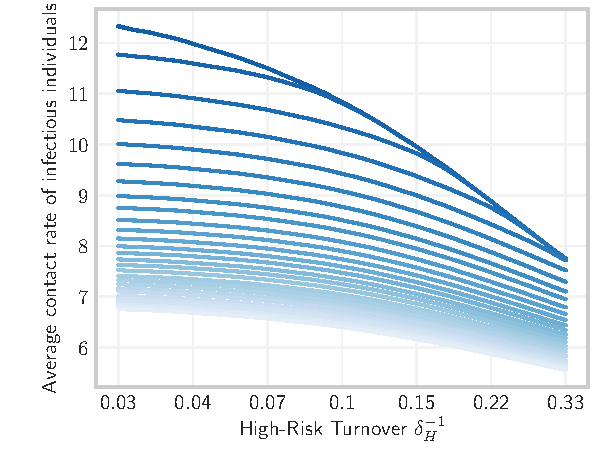
\includegraphics[width=\linewidth]{2d-C-I}
    \caption{Average contact rate among infectious individuals $\hat{C}_{\mathcal{I}}$}
    \label{fig:2d-C-I}
  \end{subfigure}
  \begin{subfigure}[t]{0.45\linewidth}
    \centering
    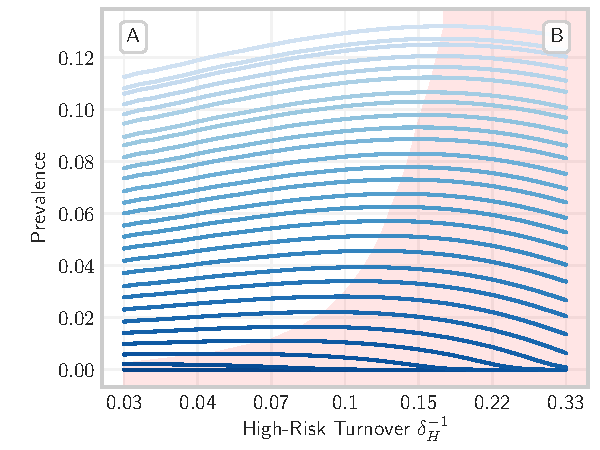
\includegraphics[width=\linewidth]{2d-prevalence-all}
    \caption{Overall prevalence $\hat{\mathcal{I}}$}
    \label{fig:2d-prevalence-all}
  \end{subfigure}\\[1em]
  \begin{subfigure}[t]{0.45\linewidth}
    \centering
    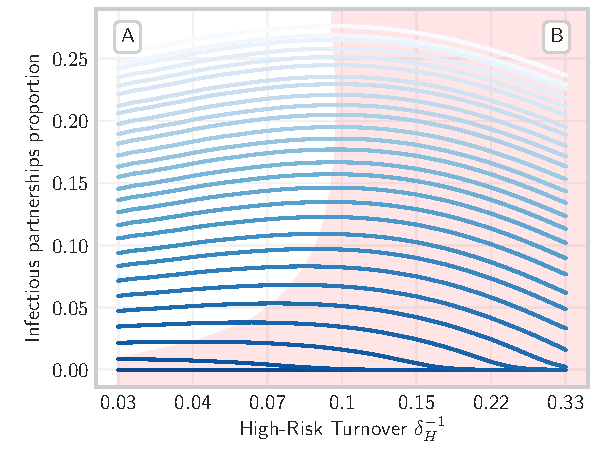
\includegraphics[width=\linewidth]{2d-XC-I}
    \caption{Proportion of available partnerships
      which are offered by infectious individuals $\bm{C}_{\mathcal{I}}$}
    \label{fig:2d-XC-I}
  \end{subfigure}
  \begin{subfigure}[t]{0.45\linewidth}
    \centering
    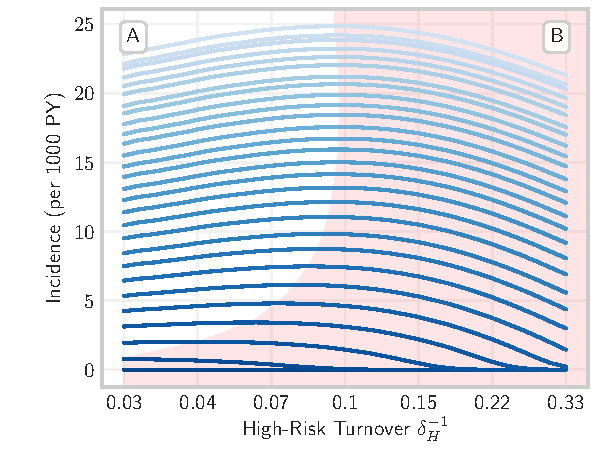
\includegraphics[width=\linewidth]{2d-incidence-all}
    \caption{Overall incidence $\lambda$}
    \label{fig:2d-incidence-all}
  \end{subfigure}
  \caption{Incidence and the dynamic factors of incidence versus turnover,
    for a range of treatment rates.
    Darker blue indicates higher treatment rate.
    The product of components (a) and (b) is proportional to
    (c) the proportion of total available contacts which are with infectious individuals
    and (d) overall incidence.}
  \label{fig:2d-incidence-factors}
\end{figure}
\par
Finally, Figure~\ref{fig:surface} summarizes trends in
overall equilibrium incidence and group-specific prevalence
with respect to both turnover $\phi$ and treatment rate $\tau$.%
\footnote{Figures~\ref{fig:surface-prevalence-all}~and~\ref{fig:surface-incidence-all}
  are the surface projections of the profiles shown in
  Figures~\ref{fig:2d-prevalence-all}~and~\ref{fig:2d-incidence-all}, respectively.}
Treatment consistently decreased equilibrium incidence (as noted above),
as well as prevalence, at all rates of turnover.
As suggested in Experiment 1.2, infection prevalence increased with turnover
for moderate rates of turnover and treatment, among all groups, and overall.
However, for higher rates of turnover,
prevalence among each risk group peaked, and then declined.
As shown in Figure~\ref{fig:2d-incidence-factors},
the rate of turnover at which the peak occurs decreased with treatment rate.
Finally, for high rates of treatment and/or turnover, the product of
the average contact rate of infectious individuals $\hat{C}_\mathcal{I}$
and prevalence $\hat{\mathcal{I}}$
was too low to sustain the epidemic.
That is, the basic reproductive number $R_0$ declined to less than one,
and no epidemic was  observed.%
\footnote{In fact, it can be shown that for extreme rates of turnover,
  a heterogeneous system (e.g. Full model) will converge on
  a homogeneous system (e.g. model V1).
  This result is shown in Figure~\ref{fig:hetero-converge}.}
\begin{figure}[!tbp]
  \centering
  \begin{subfigure}{0.45\linewidth}
    \centering
    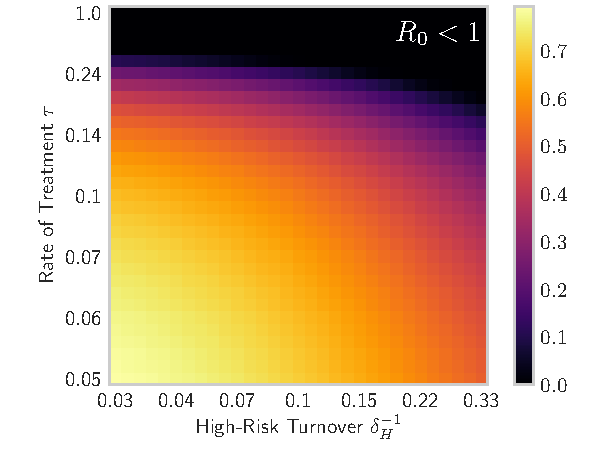
\includegraphics[width=\linewidth]{surface-prevalence-high}
    \caption{High risk prevalence}
    \label{fig:surface-prevalence-high}
  \end{subfigure}
  \begin{subfigure}{0.45\linewidth}
    \centering
    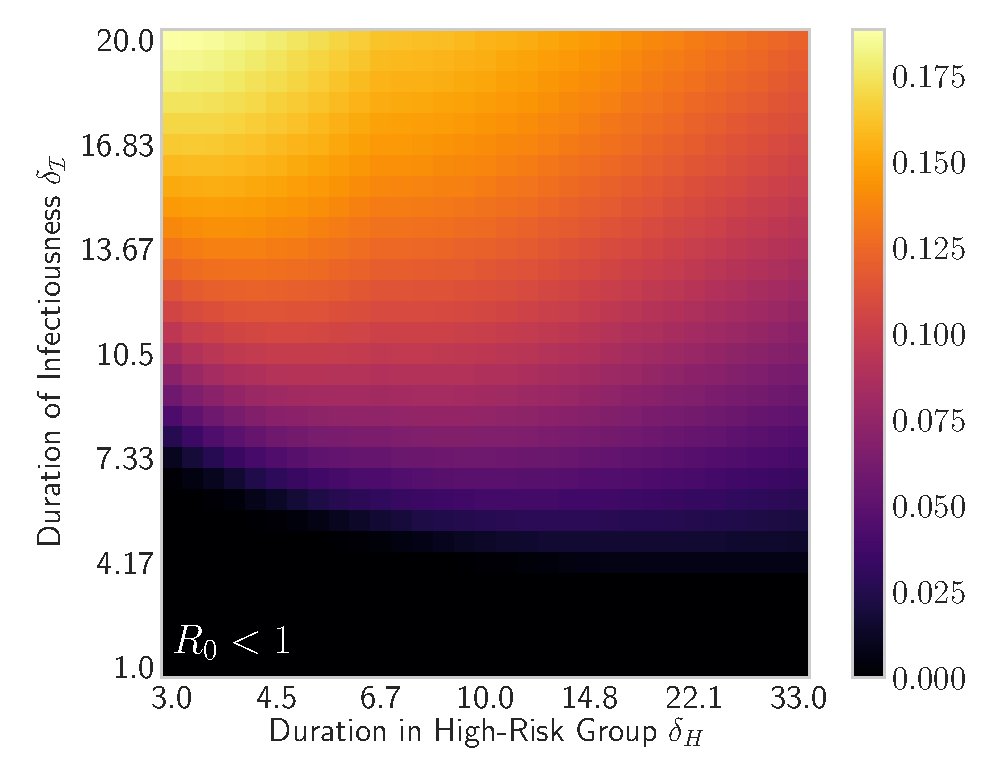
\includegraphics[width=\linewidth]{surface-prevalence-low}
    \caption{Low risk prevalence}
    \label{fig:surface-prevalence-low}
  \end{subfigure}\\[1em]
  \begin{subfigure}{0.45\linewidth}
    \centering
    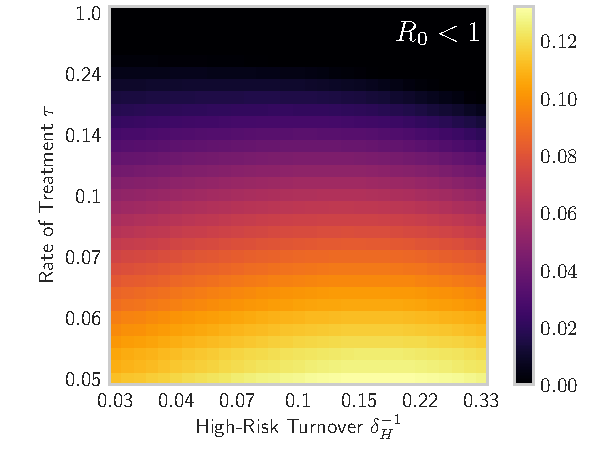
\includegraphics[width=\linewidth]{surface-prevalence-all}
    \caption{Overall prevalence}
    \label{fig:surface-prevalence-all}
  \end{subfigure}
  \begin{subfigure}{0.45\linewidth}
    \centering
    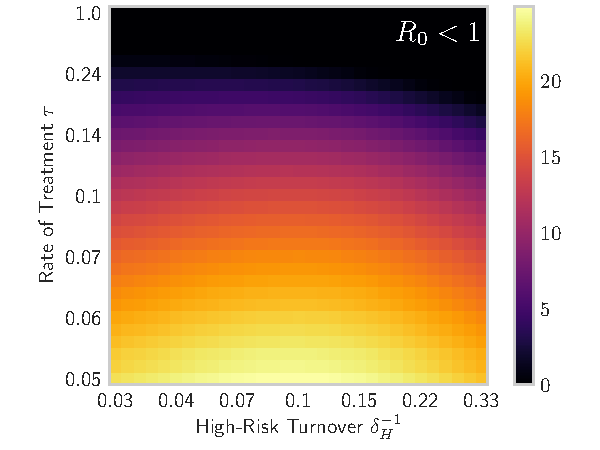
\includegraphics[width=\linewidth]{surface-incidence-all}
    \caption{Overall incidence}
    \label{fig:surface-incidence-all}
  \end{subfigure}
  \caption{Equilibrium prevalence and incidence for different rates of
    turnover $\phi$ (log scale) and
    treatment $\tau$ (log scale).}
  \label{fig:surface}
\end{figure}
% ==================================================================================================
\subsection{Experiment 2: Inferred risk heterogeneity with vs without turnover}
\label{ss:res-infer}
Before model fitting, the predicted prevalence ratio
between high and low risk groups was lower with turnover than without:
$\input{\datapath/values/turnover-prevalence-ratio.txt}$~vs~%
$\input{\datapath/values/no-turnover-prevalence-ratio.txt}$.
This reflects the ``homogenizing'' effect of turnover on
the average risk experienced by individuals in the model.
As shown in Figure~\ref{fig:2d-ratio-prevalence-high-low},
the high-to-low prevalence ratio consistently declined with turnover
for all turnover and treatment rates explored.
Thus, when fitting the model to target prevalence values,
the fitted contact rates $C$ would have to compensate for this difference.
\par
After fitting the contact rates, both models predicted
the desired equilibrium infection prevalence values of 20\%,~3\%,~and~5\%
among the high risk group, low risk group, and overall.
However, in order to do so, the ratio of fitted contact rates
between high and low risk groups ($C_H~/~C_L$)
was higher with turnover than without:
$\input{\datapath/values/turnover-[fit]-C-ratio.txt}$~vs~%
$\input{\datapath/values/no-turnover-[fit]-C-ratio.txt}$.
That is, the inferred level of risk heterogeneity was higher
in the model with turnover than in the model without turnover.
This is because,
in order to observe the same prevalence ratio in a system with turnover,
the ``risk homogenizing'' effects of turnover must be overcome by
greater heterogeneity in risk, as compared to a system without turnover.
These results are also summarized in Table~\ref{tab:fitting}.
\begin{table}
  \centering
  \caption{Equilibrium contact rates $C$ and prevalence $P$
    among the high $H$ and low $L$ risk groups
    predicted by the models with and without turnover,
    before and after model fitting.}
  \label{tab:fitting}
  \begin{tabularx}{0.7\linewidth}{r *{6}{Y}}
	\toprule
  Model & $C_H$ & $C_L$ & $C_H~/~C_L$ & $P_H$ & $P_L$ & $P_H~/~P_L$\\\midrule
  Base &
    \input{\datapath/fit/Base-C-high.txt}
  & \input{\datapath/fit/Base-C-low.txt}
  & \input{\datapath/fit/Base-C-ratio.txt}
  & \input{\datapath/fit/Base-prevalence-high.txt}
  & \input{\datapath/fit/Base-prevalence-low.txt}
  & \textbf{\input{\datapath/fit/Base-prevalence-ratio.txt}}\\
  V3 &
    \input{\datapath/fit/V3-C-high.txt}
  & \input{\datapath/fit/V3-C-low.txt}
  & \input{\datapath/fit/V3-C-ratio.txt}
  & \input{\datapath/fit/V3-prevalence-high.txt}
  & \input{\datapath/fit/V3-prevalence-low.txt}
  & \textbf{\input{\datapath/fit/V3-prevalence-ratio.txt}}\\
  Base [fit] &
    \input{\datapath/fit/Base-fit-C-high.txt}
  & \input{\datapath/fit/Base-fit-C-low.txt}
  & \textbf{\input{\datapath/fit/Base-fit-C-ratio.txt}}
  & \input{\datapath/fit/Base-fit-prevalence-high.txt}
  & \input{\datapath/fit/Base-fit-prevalence-low.txt}
  & \input{\datapath/fit/Base-fit-prevalence-ratio.txt}\\
  V3 [fit] &
    \input{\datapath/fit/V3-fit-C-high.txt}
  & \input{\datapath/fit/V3-fit-C-low.txt}
  & \textbf{\input{\datapath/fit/V3-fit-C-ratio.txt}}
  & \input{\datapath/fit/V3-fit-prevalence-high.txt}
  & \input{\datapath/fit/V3-fit-prevalence-low.txt}
  & \input{\datapath/fit/V3-fit-prevalence-ratio.txt}\\
  \bottomrule
\end{tabularx}
\end{table}
% ==================================================================================================
\subsection{Experiment 3: Influence of turnover on the TPAF of the high risk group}
\label{ss:res-tpaf}
Finally, we compared the predicted TPAF of the high risk group with and without turnover in:
two settings (same parameters, different prevalence); and
two models (same prevalence, different parameters).
These results are shown in Figure~\ref{fig:tpaf}.
The TPAF approaches 1 for all models over the 50 year period,
indicating that unmet treatment needs of the high risk group
are central to epidemic persistence in all scenarios.
Additionally, no TPAFs intersect during this period,
so relative differences between TPAFs can be described irrespective of time horizon.
\begin{figure}[!tbp]
  \centering
  \begin{subfigure}{0.45\linewidth}
    \centering
    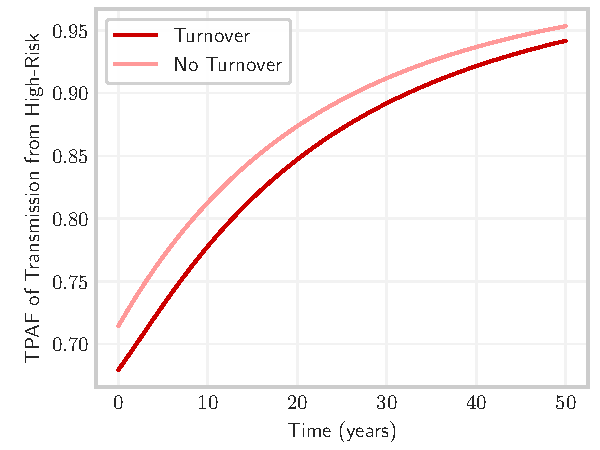
\includegraphics[width=\linewidth]{sit-tpaf-tpaf-high-all-vs=raw}
    \caption{No fitting}
    \label{fig:tpaf-raw}
  \end{subfigure}
  \begin{subfigure}{0.45\linewidth}
    \centering
    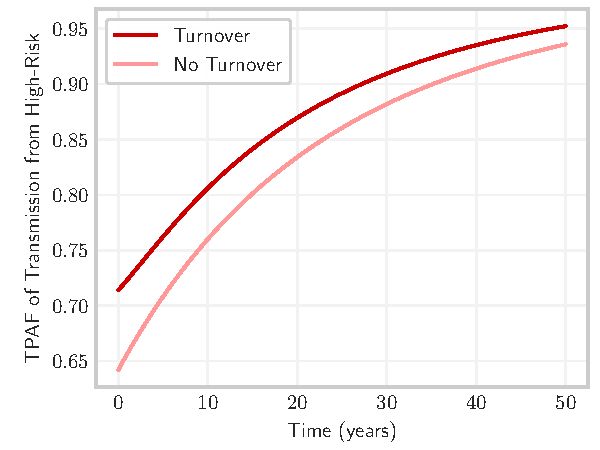
\includegraphics[width=\linewidth]{sit-tpaf-tpaf-high-all-vs=fit}
    \caption{Fitted contact rates}
    \label{fig:tpaf-fit}
  \end{subfigure}
  \caption{Transmission population attributable fraction (TPAF-from)
    of the high risk group with and without turnover,
    and with and without fitted contact rates to group-specific prevalence.}
  \label{fig:tpaf}
\end{figure}
% --------------------------------------------------------------------------------------------------
\paragraph{Experiment 3.1: Two settings}
\label{p:res-tpaf-raw}
Figure~\ref{fig:tpaf-raw} shows the estimated TPAF of the high risk group
in two different settings -- with and without turnover.
In this case, the estimated TPAF is lower
in Setting B with turnover versus
in Setting A without turnover.
This can be attributed to
the larger equilibrium prevalence ratio without model fitting
(Experiment 2, Table~\ref{tab:fitting}),
which results in more onward transmission from the high prevalence high risk group.
In other words, the importance of reaching the high risk group
in a context without turnover is higher than in a context with turnover,
all other factors being equal.
% --------------------------------------------------------------------------------------------------
\paragraph{Experiment 3.2: Two models}
\label{p:res-tpaf-fit}
Figure~\ref{fig:tpaf-fit} shows the estimated TPAF of the high risk group
by two different models -- with and without turnover --
both fitted to the same prevalence.
Now the estimated TPAF is higher
in Model B with turnover versus
in Model A without turnover.
This result, opposite to Experiment 3.1, can be explained by two factors.
First, the equilibrium prevalence ratios predicted by the models with and without turnover
are equalized through model fitting to the same targets.
As a result, differences in prevalence in the high risk group
no longer contribute to an increased TPAF estimate by Model A without turnover.
Second, as shown in Experiment 2, 
the ratio of fitted contact rates $C_H~/~C_L$ in model B with turnover
are higher than in Model A without.
This affords a higher risk of onward transmission to the high risk group
in Model B with turnover, and thus an increased TPAF.
This result then implies that
models which fail to capture turnover dynamics which are present in reality
may underestimate the TPAF of high risk groups.
Consequently, the importance of prioritizing high risk groups
to achieve epidemic control may be similarly underestimated by such models.
%% SS: This section perhaps could be a bit clearer as clearly very important
%% Is there a way to more explicitly talk about new infections
%% in the low / medium risks coming from prevalent infections
%% entering into these states from high risk groups and that
%% subsequent infections emanating from these individuals are thus still
%% linked back to prior history in the high risk group? 
